\section{Software Implementation}
SciKit-SurgeryFRED implements a simple user interface, Figure \ref{fig:surgery_fred}, to demonstrate registration of a pre-operative image to intra-operative space. At startup a target is placed at a random location within the pre-operative image, shown as a red circle. The standard deviation of the \gls{FLE} is randomly sampled from a uniform distribution 

\begin{figure}
	\begin{center}
	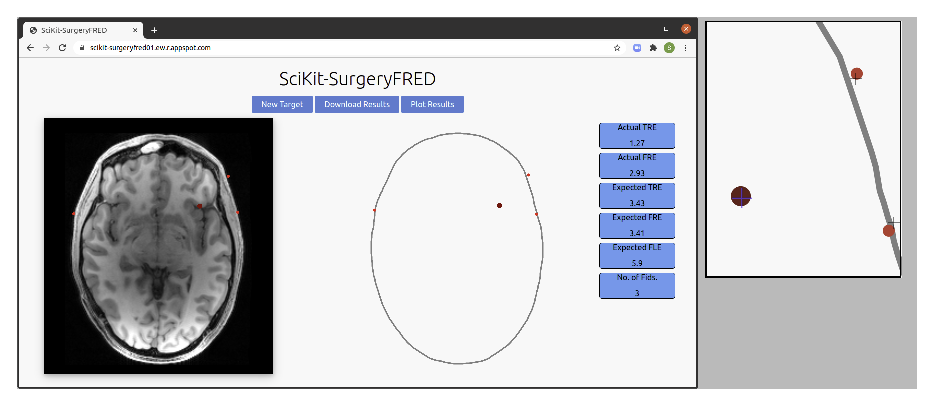
\includegraphics[width=0.9\linewidth]{scikit-surgeryfred_gui.eps}
		\caption{\label{fig:surgery_fred}SciKit-SurgeryFRED graphical user interface after 3 fiducial markers placed. The red sphere in the pre-operative image (left) represents a clinical target, which is located in the
		intra-operative space (middle) by fiducial based registration, using the fiducial markers (green). FLE is added to each marker in the intra-operative image, this is more clearly visible on the zoomed in images at the right. The resulting registration results in a TRE, shown by the misalignment of the red circle and crosshair 
		on the enlarged image at right. TRE and other statistics are shown across the top
		of the window.}
	\end{center}
\end{figure}


